\section{Magnetic Resonance Imaging: A Preview}

\subsection{Summary}
\begin{enumerate}
    \item The name \textbf{MRI}
    \begin{itemize}
        \item \textbf{M}agnetic - the use of magnetic fields in the field
        \item \textbf{R}esonance - the need to match the frequency of an oscillating magnetic field to the precessional frequency of the spins of some nucleus
        \item \textbf{I}maging
    \end{itemize}

    \item \textbf{MRI} Concepts
    \begin{itemize}
        \item Based on the \textit{interaction of a nuclear spin with an external magnetic field $\vec{B_0}$}
        \item Precession - \textit{the circular motion of the axis of rotation of a spinning body about another fixed axis caused by the application of a torque in the direction of the precession}
        \item Imaging - based on the \textit{bulk precession of the hydrogen spins about the field direction} (Figure~\ref{fig:fig11})
        \item Precession angular frequency (Larmor Equation): \\
            \begin{equation} 
                \omega_0 = \gamma B_0
            \end{equation}

            where:
            \begin{conditions}
                \gamma & gyromagnetic ratio ($2.68 \times 10^8 rad/s/tesla$)
            \end{conditions}

        \item The Boltzmann Distribution shows that the spins can align both parallel and antiparallel with to the magnetic field. The spin excess is very small: \\
            \begin{equation} 
                \text{spin excess } \simeq N \frac{\hbar \omega_0}{2kT}
            \end{equation}

            where:
            \begin{conditions}
                N & total number of spins present in the sample \\
                k & Boltzmann constant \\
                kT & average thermal energy 
            \end{conditions}

        \item $M_0$ - the average magnetic dipole density (longitudinal equilibrium relaxation)
            \begin{equation}
                M_0 = \frac{\rho_0 \gamma^2 \hbar^2}{4kT} B_0
            \end{equation}
           
        \item $\vec{M}$ has been rotated by an rf pulse to a direction orthogonal to $\vec{B_0} = B_0 \hat{z}$. The resulting transvserse magnetization has magnitude $M_0$ and precesses clockwise in the x-y plane. The complex magnetization is:
            \begin{equation}
                M_+(t) \equiv M_x(t) + i M_y(t) = M_0 e^{-i \omega t + i \phi_0}
            \end{equation}
    \end{itemize}
\end{enumerate}

\begin{figure}[H]
	\centering
	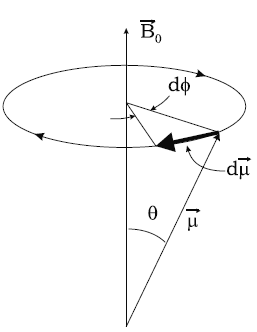
\includegraphics[width=0.4\textwidth,keepaspectratio]{fig11}
	\caption{
By definition, precession is the circular motion of the axis of rotation of a spinning body
about another fixed axis caused by the application of a torque in the direction of the precession.
The interaction of the proton's spin with the magnetic field produces the torque, causing it to
precess about $\vec{B_0}$ as the fixed axis. When looking down from above the vector $\vec{B_0}$, the precession
of the magnetic moment vector $\vec{\mu}$, which is proportional to the spin vector, is clockwise. For the
customary counterclockwise definition of polar angles, the differential $d\phi$ shown is negative.}
	\label{fig:fig11}
\end{figure}

\begin{figure}[H]
	\centering
	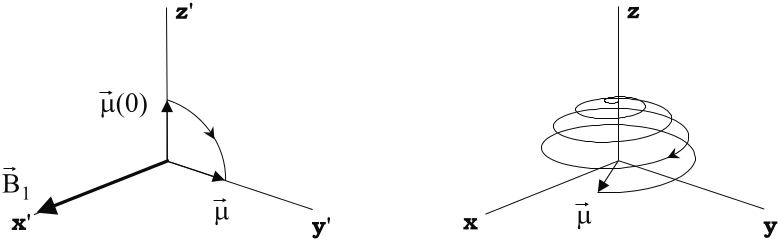
\includegraphics[width=0.7\textwidth,keepaspectratio]{fig12}
	\caption{
Illustration of the effect of an rf pulse on an individual magnetic moment $\mu$. \\
(a) In a frame rotating about $B_0$ (which is along $\hat{z}$, say) at the Larmor frequency (with coordinates
x', y' and z' = z), there is no observed precession about $B_0$. Upon application of an rf magnetic
field pulse applied along $\hat{x}'$, the magnetic moment is rotated about $\hat{x}'$ at a rate corresponding to
the frequency $\omega_1 = \gamma B_1$ determined by the amplitude of the rf field, $B_1$. A $\pi/2$ flip
relative to its starting position along $\hat{z}'$ is achieved in a 
time $\tau_{rf}$ provided that $\omega_1 \tau_{rf} = \pi/2$.\\
(b) The behavior of the same magnetic moment rotation is observed to be more complicated in the fixed laboratory
frame. This picture has been constructed for the case $\omega_1 = 0.06 \omega_0$. In actual MR applications, the
frequency $\omega_1$ would be much smaller in relation to $\omega_0$, but then the spiraling would be too dense
to illustrate.
}
	\label{fig:fig12}
\end{figure}

\begin{figure}[H]
	\centering
	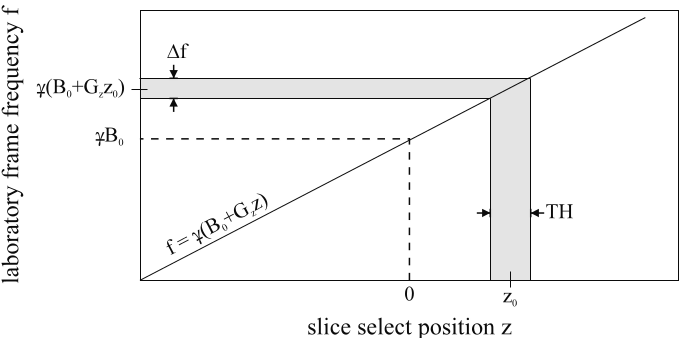
\includegraphics[width=0.7\textwidth,keepaspectratio]{fig13}
	\caption{
The precession frequency ($f = \omega/(2\pi)$) in the laboratory frame is a function of position
along the slice select axis. The original static field $B_0$ has been supplemented with a field with
constant gradient $G_z$ in the z-direction. The central frequency and spectral bandwidth of the rf
pulse ($\Delta f \equiv BW_{rf}$, the shaded horizontal strip) are such that the slice of thickness 
$\Delta z \equiv T H$ (the
shaded vertical strip) is uniformly 'excited' (i.e., all spins in the slice have the resonance condition
satisfied). The fact that the slice is offset from the origin in the z-direction by $z_0$ implies that the
center frequency of the rf pulse must be offset from the static Larmor frequency $f_0 = \gammabar B_0$ by $\gammabar G_z z_0$ as has been shown along the frequency axis. }
	\label{fig:fig13}
\end{figure}

\begin{figure}[H]
	\centering
	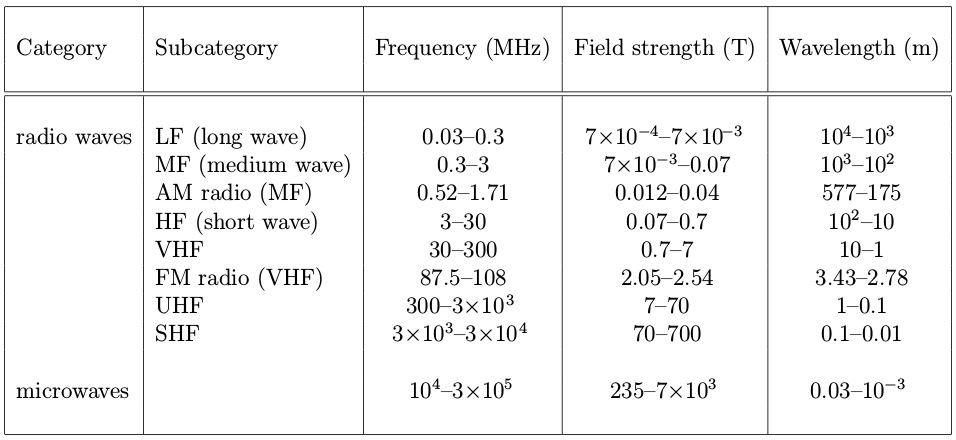
\includegraphics[width=0.8\textwidth,keepaspectratio]{tab11}
	\caption{
Range of radio and microwave frequencies from Wikipedia at en.wikipedia.org. Under
the subcategory heading, the letter F refers to frequency. The letters L, M, H, V, U, and S in front
of the letter F refer to low, medium, high, very, ultra, and super, respectively. Associated free-space
wavelengths and NMR field strengths for protons are given here.
}
	\label{fig:tab11}
\end{figure}
